%

\documentclass[twoside]{article}
\usepackage{graphics}
\usepackage{amsmath}
\setlength{\oddsidemargin}{0.25 in}
\setlength{\evensidemargin}{-0.25 in}
\setlength{\topmargin}{-0.6 in}
\setlength{\textwidth}{6.5 in}
\setlength{\textheight}{8.5 in}
\setlength{\headsep}{0.75 in}
\setlength{\parindent}{0 in}
\setlength{\parskip}{0.1 in}

%
% The following commands set up the lecnum (lecture number)
% counter and make various numbering schemes work relative
% to the lecture number.
%
\newcounter{lecnum}
\renewcommand{\thepage}{\thelecnum-\arabic{page}}
\renewcommand{\thesection}{\thelecnum.\arabic{section}}
\renewcommand{\theequation}{\thelecnum.\arabic{equation}}
\renewcommand{\thefigure}{\thelecnum.\arabic{figure}}
\renewcommand{\thetable}{\thelecnum.\arabic{table}}

%
% The following macro is used to generate the header.
%
\newcommand{\lecture}[4]{
   \pagestyle{myheadings}
   \thispagestyle{plain}
   \newpage
   \setcounter{lecnum}{#1}
   \setcounter{page}{1}
   \noindent
   \begin{center}
   \framebox{
      \vbox{\vspace{2mm}
    \hbox to 6.28in { {\bf EE 382V: Social Computing
                        \hfill Fall 2018} }
       \vspace{4mm}
       \hbox to 6.28in { {\Large \hfill Scribe Assignment #1: #2  \hfill} }
       \vspace{2mm}
       \hbox to 6.28in { {\it Lecturer: #3 \hfill Scribe: #4} }
      \vspace{2mm}}
   }
   \end{center}
   \markboth{Lecture #1: #2}{Lecture #1: #2}
   %{\bf Disclaimer}: {\it These notes have not been subjected to the
   %usual scrutiny reserved for formal publications.  They may be distributed
   %outside this class only with the permission of the Instructor.}
   \vspace*{4mm}
}

%
% Convention for citations is authors' initials followed by the year.
% For example, to cite a paper by Leighton and Maggs you would type
% \cite{LM89}, and to cite a paper by Strassen you would type \cite{S69}.
% (To avoid bibliography problems, for now we redefine the \cite command.)
% Also commands that create a suitable format for the reference list.
\renewcommand{\cite}[1]{[#1]}
\def\beginrefs{\begin{list}%
        {[\arabic{equation}]}{\usecounter{equation}
         \setlength{\leftmargin}{2.0truecm}\setlength{\labelsep}{0.4truecm}%
         \setlength{\labelwidth}{1.6truecm}}}
\def\endrefs{\end{list}}
\def\bibentry#1{\item[\hbox{[#1]}]}

%Use this command for a figure; it puts a figure in wherever you want it.
%usage: \fig{NUMBER}{SPACE-IN-INCHES}{CAPTION}
\newcommand{\fig}[3]{
			\vspace{#2}
			\begin{center}
			Figure \thelecnum.#1:~#3
			\end{center}
	}
% Use these for theorems, lemmas, proofs, etc.
\newtheorem{theorem}{Theorem}[lecnum]
\newtheorem{lemma}[theorem]{Lemma}
\newtheorem{proposition}[theorem]{Proposition}
\newtheorem{claim}[theorem]{Claim}
\newtheorem{corollary}[theorem]{Corollary}
\newtheorem{definition}[theorem]{Definition}
\newenvironment{proof}{{\bf Proof:}}{\hfill\rule{2mm}{2mm}}

% **** IF YOU WANT TO DEFINE ADDITIONAL MACROS FOR YOURSELF, PUT THEM HERE:

\begin{document}
%FILL IN THE RIGHT INFO.
%\lecture{**LECTURE-NUMBER**}{**DATE**}{**LECTURER**}{**SCRIBE**}
\lecture{1}{September 29}{Vijay Garg}{Zach Southwell}
%\footnotetext{These notes are partially based on those of Nigel Mansell.}

\section{The LP formulation of Max-Flow Min-Cut problem}
\subsection{Problem Domain}
We are given a connected graph which is directed from an origin node $s$ to a destination node $t$, where each edge in the graph has some non-negative capacity which represents the maximum flow across the edge.
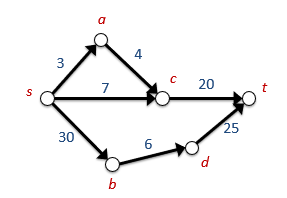
\includegraphics{mfmc1.png}

\fig{1}{0pt}{sample flow}
\subsection{Primal Problem}
We want to calculate the {\em maximum flow} which can be sent from $s$ to $t$. Another way to state this is that we want to maximize the flow through each edge from $s$ subject to these constraints:
\begin{itemize}
    \item Conservation constraints: The size of a the incoming flow for a vertex must be the same as the outgoing flow
    \item Capacity constraints: No edge may carry more than its maximum capacity. Define $c(u,v)$ as the maximum capacity for an edge $(u,v) \in E$
    \item The flow through each edge must be non-negative
\end{itemize}
\newpage
This can be stated as the following linear program:\\\\
Maximize:
$$\sum_{v: (s,v) \in E}f(s,v)$$\\
Subject to: \\
$$
\begin{gathered}
\sum_{u: (u,v) \in E}f(u,v) = \sum_{w: (v,w) \in E}f(v,w)\\
f(u,v) \leq c(u,v)\qquad \forall(u,v) \in E\\
f(u,v) \geq 0\qquad \forall(u,v) \in E
\end{gathered}
$$

\subsection{Dual Problem}
The dual problem is to {\em cut} the graph into two components with one containing $s$ and the other containing $t$ by removing the edges with the minimum total capacity. Let $S$ be the component containing $s$ and $T$ be the component containing $t$. Every node in the graph (except for $s$ and $t$) has a dual variable $y(u)$ which is 1 if $u \in S$ and 0 otherwise, and every edge in the graph has a dual variable $y(u,v)$ which is 1 if $u \in S$ and $v \in T$ and 0 otherwise.  The dual problem can be stated as:\\\\
Minimize:
$$\sum_{(u,v) \in E}c(u,v)*y(u,v)$$\\
Subject to: \\
$$
\begin{gathered}
y(v) + y(s,v) \geq 1\qquad \forall v: (s,v) \in E\\
y(v) - y(u) + y(u,v) \geq 0\qquad \forall(u,v) \in E (s \neq u, t \neq v)\\
-y(u) + y(u,t) \geq 0\qquad \forall u: (u,t) \in E
\end{gathered}
$$
\newpage
\subsection{Primal Example}
For figure 1.1, the primal problem can be stated as:\\\\
Maximize:
$$f(s,a) + f(s,c) + f(s,b)$$
Subject to:\\
$$
\begin{gathered}
f(s,a) - f(a,c) = 0\\
f(s,b) - f(b,d) = 0\\
f(a,c) + f(s,c) - f(c,t) = 0\\
f(b,d) - f(d,t) = 0\\
f(s,a) \leq3\\
f(s,c) \leq7\\
f(s,b) \leq30\\
f(a,c) \leq4\\
f(b,d) \leq6\\
f(c,t) \leq20\\
f(d,t) \leq25\\
f(u,v) \geq 0\qquad \forall(u,v) \in E
\end{gathered}
$$

\subsection{Dual Example}
Minimize:
$$c(s,a)*y(s,a) + c(s,b)*y(s,b) + c(s,c)*y(s,c) + c(a,c)*y(a,c) + c(b,d)*y(b,d) + c(c,t)*y(c,t) + c(d,t)*y(d,t)$$
Subject to:
$$
\begin{gathered}
y(a) + y(s,a) \geq 1\\
y(b) + y(s,b) \geq 1\\
y(c) + y(s,c) \geq 1\\
y(c) -y(a) + y(a,c) \geq 0\\
y(d) -y(b) + y(b,d) \geq 0\\
-y(c) + y(c,t) \geq 0\\
-y(d) + y(d,t) \geq 0\\
\end{gathered}
$$
\newpage
\subsection{Solution}
The following mapping satisfies the primal with a value of 16:
$$f(s,a)=3; f(s,c)=7; f(s,b)=6; f(a,c)=3; f(c,t)=10; f(b,d)=6; f(d,t)=6$$

And the following `cut' satisfies the dual with a value of 16:
$$y(s,a)=1; y(s,c)=1; y(s,b)=0; y(a,c)=0; y(c,t)=0; y(b,d)=1; y(d,t)=0$$

Since the primal and dual solutions have the same value, we know that these solutions are optimal.

A value of 1 for $y(s,a), y(s,c), y(b,c)$ in the dual problem indicates that the edge belongs to the `cut' set. Finding these constraining edges is the intuitive and natural approach to solving the maximization problem. This is interesting because even without formal knowledge of LP duality in this case, you would have a tendency to construct the dual in order to solve the primal problem.
\end{document}